\documentclass{article}

\usepackage{amsmath}
\usepackage{graphicx}
\usepackage{titlesec}
\usepackage[T1,T2A]{fontenc}
\usepackage[utf8]{inputenc}
\usepackage[english,russian]{babel}

\titleformat{\section}
            {\normalfont\Large\bfseries}
            {}
            {0pt}
            {Урок \thesection\quad}

\begin{document}

\noindent\makebox[\textwidth]{\rule{\paperwidth}{0.4pt}}
\section{(08.09.2018)}
\noindent\makebox[\textwidth]{\rule{\paperwidth}{0.4pt}}

\subsection{Магнитное поле}

\paragraph{}

Магнитное поле порождается движущимися электрическими зарядами (током).

\paragraph{}

\textbf{Индукция магнитного поля $\vec{B}$} - векторная величина, являющаяся силовой характеристикой магнитного поля.
Определяет, с какой силой поле $\vec{F}$ действует на заряд $q$, движущийся со скоростью $\vec{v}$.

\begin{equation*}
  \vec{F} = q[\vec{v} \times \vec{B}], \quad\quad \vec{B} = [\textup{Тл}]
\end{equation*}
\paragraph{}

Пусть мы переходим из одной системы отсчёта в другую.
Из преобразований Лоренца следует, что:

\begin{equation*}
  F_1 = F_0\sqrt{1-\frac{\upsilon^2}{c^2}},
\end{equation*}
\paragraph{}

где $F_0$ - сила в покое, $\upsilon$ - скорость системы отсчета.

\paragraph{}

Пусть два заряда покоятся. По закону Кулона

\begin{equation*}
  F_0 = \frac{1}{4\pi\varepsilon_0}\frac{q_1q_2}{r^2}
\end{equation*}
\paragraph{}

Перейдем в систему отсчета, движущуюся со скоростью $\upsilon$.\\ Найдем \textbf{обобщенную силу Лоренца}:

\begin{equation*}
  F_1 = \frac{1}{4\pi\varepsilon_0}\frac{q_1q_2}{r^2}
  \frac{\big( \sqrt{1-\frac{\upsilon^2}{c^2}} \big)^2}{\sqrt{1-\frac{\upsilon^2}{c^2}}} =
  \underbrace{\frac{1}{4\pi\varepsilon_0r^2}\frac{q_1q_2}{\sqrt{1-\frac{\upsilon^2}{c^2}}}}_{F_\textup{электр.}} -
  \frac{\upsilon^2}{c^2}\underbrace{\frac{q_1q_2}{\sqrt{1-\frac{\upsilon^2}{c^2}}}}_{F_\textup{магн.}}
\end{equation*}

Отсюда следует, что
\begin{equation*}
  \frac{F_{\textup{магн.}}}{F_{\textup{электр.}}} = \frac{\upsilon^2}{c^2}.
\end{equation*}
\paragraph{}

Перепишем формулу для силы магнитного взаимодействия:

\begin{equation*}
  F_M = \frac{uq_1}{4\pi\varepsilon_0r^2c^2}\frac{uq_2}{\sqrt{1-\frac{\upsilon^2}{c^2}}}
\end{equation*}
\paragraph{}

Введём индукцию магнитного поля B

\begin{equation*}
  B = \frac{uq_2}{4\pi\varepsilon_0c^2r^2\sqrt{1-\frac{\upsilon^2}{c^2}}}
\end{equation*}
\paragraph{}
Тогда формула силы магнитного взаимодействия запишется следующим образом:

\begin{equation*}
  F_M = q_1\upsilon B
\end{equation*}
\paragraph{}

Её можно трактовать так: заряд $q_2$ создаёт поле и действует на заряд $q_1$ с силой $F_M$.

\paragraph{}

Для удобства введём константу $\mu_0$:

\begin{equation*}
  \mu_0 = \frac{1}{\varepsilon_0c^2}
\end{equation*}
\paragraph{}

Тогда формула для магнитной индукции

\begin{equation*}
  B = \frac{\mu_0}{4\pi}\frac{uq}{r^2\sqrt{1-\frac{\upsilon^2}{c^2}}}
\end{equation*}
\paragraph{}

\textbf{Сила Ампера} --- сумма сил Лоренца от нескольких зарядов

\begin{equation*}
  F_A = BIL
\end{equation*}

\newpage

\paragraph{}
Пусть есть бесконечный заряженный провод и заряд $Q$ на расстоянии $x$ от провода. $S$ --- площадь
сечения провода, $\rho$ --- объемная плотность заряда.
\paragraph{}
\noindent\makebox[\textwidth][c]{
\begin{minipage}{0.6\textwidth}
  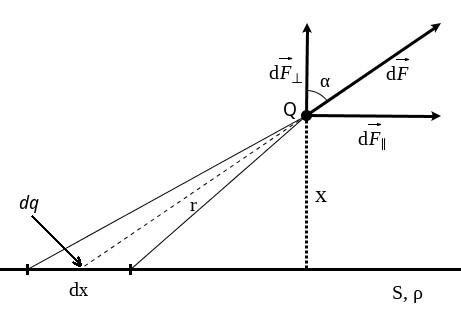
\includegraphics[width=\linewidth,natwidth=461,natheight=316]{images/1.jpg}
\end{minipage}}
\paragraph{}

\begin{equation*}
  dF_\parallel = dFsin\alpha, \quad dF_\perp = dFcos\alpha, \quad dq = \rho Sdx
\end{equation*}

\begin{equation*}
  dF = \frac{1}{4\pi\varepsilon_0}\frac{Q\rho Sdx}{r^2}, \quad r = \frac{x}{cos\alpha},
  \quad dx = \frac{rd\alpha}{cos\alpha}
\end{equation*}

\begin{equation*}
  dF_\perp = \frac{1}{4\pi\varepsilon_0}\frac{Q\rho Sdx}{x^2}cos^2\alpha cos\alpha
\end{equation*}
\paragraph{}

Подставим $r$, $dx$ и проинтегрируем:

\begin{equation*}
  F_\perp = \int_{-\frac{\pi}{2}}^{\frac{\pi}{2}}\frac{1}{4\pi\varepsilon_0}\frac{Q\rho Scos\alpha}{x}d\alpha =
  \frac{Q\rho S}{2\pi\varepsilon_0x}
\end{equation*}
\paragraph{}

Перейдем в систему отсчёта, движущуюся вправо со скоростью $\upsilon$:

\begin{equation*}
  F' = F_0\sqrt{1-\frac{\upsilon^2}{c^2}}, \quad F_M = -\frac{\upsilon^2}{c^2}\frac{Q\rho S}
  {2\pi\varepsilon_0x\sqrt{1-\frac{\upsilon^2}{c^2}}}
\end{equation*}

\newpage

Рассмотрим ток в проводнике с поперечным сечением $S$. Пусть средняя скорость электронов $u$,
$n$ --- объемная концентрация электронов.

\paragraph{}
\noindent\makebox[\textwidth][c]{
  \begin{minipage}{0.6\textwidth}
    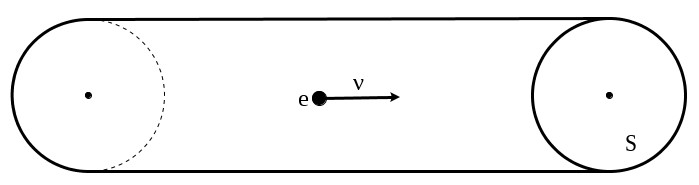
\includegraphics[width=\linewidth,natwidth=699,natheight=185]{images/2.jpg}
\end{minipage}}
\paragraph{}

\begin{equation*}
  I = \frac{\Delta q}{\Delta t} = \frac{enSu\Delta t}{\Delta t} = neSu
\end{equation*}
\paragraph{}

Перепишем формулу $F_M$:

\begin{equation*}
  F_M = -uQ\frac{\mu_0}{2\pi}\frac{\rho S\upsilon}{x\sqrt{1-\frac{\upsilon^2}{c^2}}}
\end{equation*}
\paragraph{}

Но так как $\rho S\upsilon = neS\upsilon = I$, имеем

\begin{equation*}
  F_M = -uQ\frac{\mu_0}{2\pi}\frac{I}{x\sqrt{1-\frac{\upsilon^2}{c^2}}}
\end{equation*}
\paragraph{}

Мы получили формулу \textbf{силы взаимодействия заряда и бесконечного провода.}

\paragraph{}

Рассмотрим теперь случай двух проводников

\noindent\makebox[\linewidth][c]{
\begin{minipage}{0.6\linewidth}
  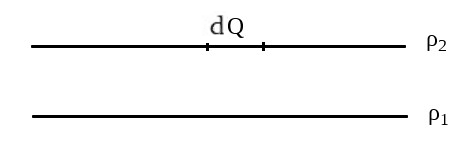
\includegraphics[width=\linewidth,natwidth=473,natheight=157]{images/3.jpg}
\end{minipage}}
\paragraph{}

\begin{equation*}
  dF_M = -\upsilon\frac{\mu_0}{2\pi} \frac{IdQ}{x\sqrt{1-\frac{\upsilon^2}{c^2}}}, \quad dQ = \rho_2Sdx_2,
  \quad dF_M = -\upsilon n_2eS\frac{\mu_0}{2\pi} \frac{I_1dx_2}{x\sqrt{1-\frac{\upsilon^2}{c^2}}}
\end{equation*}
\paragraph{}

Получим формулу \textbf{силы магнитного взаимодействия двух параллельных проводов:}

\begin{equation*}
  dF_M = -\frac{\mu_0}{2\pi} \frac{I_1I_2}{x\sqrt{1-\frac{\upsilon^2}{c^2}}} dx
\end{equation*}
\paragraph{}

Без доказательства примем на веру следующие утверждения:

\begin{equation*}
  \oint_SBds = 0, \quad \oint_lBdl = \mu_0I
\end{equation*}

Второе равенство также называется \textbf{теоремой о циркуляции:} Пусть есть замкнутый ток $I$ и взят некий контур.
Определим \textbf{циркуляцию}, как сумму всех $\vec{B}\cdot d\vec{l}$. Тогда циркуляция в этом контуре равна $\mu_0I$.

\paragraph{}

Магнитное поле является не потенциальным, а вихревым. Это значит, что его силовые линии замкнуты,
а циркуляция отлична от нуля на контуре, который охватывает ток.

\paragraph{}

Рассчитаем магнитное поле, создаваемое бесконечным проводом во всём пространстве:
\paragraph{}
\begin{minipage}{0.4\linewidth}
  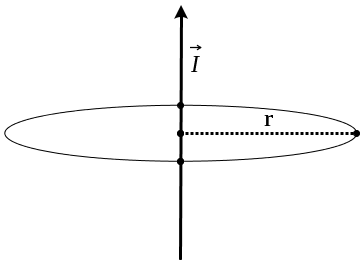
\includegraphics[width=\linewidth,natwidth=364,natheight=266]{images/4.png}
\end{minipage}
\begin{minipage}{0.5\linewidth}
  \begin{equation*}
    B2\pi r = \mu_0I \Rightarrow B = \frac{\mu_0I}{2\pi r}
  \end{equation*}
\end{minipage}

\paragraph{}

Для магнитного поля справедлив принцип суперпозиции: $\vec{B} = \Sigma\vec{B_i}$

\paragraph{Список литературы:}

\begin{itemize}
\item
  Калашников С.Г. Электричество
\item
  Зильберман Г.Е. Электричество и магнетизм
\item
  Сивухин Д.В. Общий курс физики. Т.3. Электричество
\end{itemize}

\end{document}
